
\chapter{引言}
\paragraph{这是什么？}
这些页面是一本张量导览，使用“张量图”的视觉语言。
为了展示这种方法的普适性，我尽量紧跟传奇的《Matrix Cookbook》。
因此，正文大多是关于张量及其相关内容的一组事实（恒等式、近似、不等式、关系，等等）。
你不会在这里看到太多原始手册之外的结果，但希望这些图示能为你提供一种新的理解和欣赏方式。

\paragraph{这是一个持续进行的项目：}
《Matrix Cookbook》是一本很长的书，并不是每一部分都同样适合用图示表达。
因此我选择跳过某些部分，并缩短另一些部分。
也许将来，我或其他人会进一步扩展覆盖范围。

例如，我们覆盖了关于线性组合的期望和高斯矩的全部结果，但跳过了一般多元分布那一节。
我也不得不稍微重排材料，以避免一开始就把所有记号都介绍完。

\paragraph{复数矩阵与协方差}
张量图（或张量网络）目前最常见于量子物理，
但这不是一本给物理学家的书。
《Matrix Cookbook》是一本给工程师的书，尤其是机器学习领域，而在这里复数并不常见。
没有复数，我们就不必担心复共轭，这简化了转置，也去掉了协变与逆变张量的需要。
% In particular transposing a matrix now involves taking the conjugate (flipping the sign of the imaginary part), which introduces the need for co- and contra-variant tensors.
% None of this complexity is present with standard real valued matrices, as is common e.g. in Machine Learning applications.
%For simplicity I have decided to not include these complexities.
如果你是物理学家，你大概更需要一本关于张量分析的书。

\paragraph{Tensorgrad}
张量图的符号化特性使它们非常适合符号计算。

\paragraph{张量图记号的优点：}
与其他记号相比，张量图记号有很多好处：

诸如迹、张量积或张量缩并之类的操作，都可以不借助额外记号而直接表达。
指标和张量的名称往往可以省略。这既省时又简化记号，尤其适合那些主要只是用于求和的内部指标。
复杂缩并网络所得到张量的阶数可以一眼看出：它就是未配对连线的数量。比如，一个所有连线都接上的张量网络，无论多复杂，结果都必然是一个标量。


\paragraph{词源}
“tensor” 一词源自拉丁语 tensio，意为“张力”或“伸展”，又来自动词 tendere，意为“拉伸”或“延展”。
它最早在 19 世纪中叶由 William Rowan Hamilton 在四元数研究中引入数学语境，当时它指的是四元数的模长。
后来 Gregorio Ricci-Curbastro 和 Tullio Levi-Civita 在发展张量微积分时确立了“tensor”的现代用法；这套框架把标量、向量和矩阵的概念推广到了更复杂的多维对象。~\cite{tensor_etymology_russo, hamilton_tensor}.


\tableofcontents
\clearpage


\section{张量图}
张量图是简单的图（或“网络”），其中
节点表示变量（例如向量或矩阵），边表示
缩并（例如矩阵乘法或内积）。
下表展示了一些基本操作如何用张量图写出：

\newenvironment{compress}{
  \renewcommand{\arraystretch}{0.6} % 设置数组伸展
  \setlength{\arraycolsep}{2pt}     % 设置列间距
  \vspace{.3em}
}{
  \vspace{.3em}
  \renewcommand{\arraystretch}{1}   % 环境结束后恢复默认值
  \setlength{\arraycolsep}{5pt}     % 恢复默认列间距
}

\renewcommand{\arraystretch}{2}
\noindent
%\hspace{-1em}
\vspace{.5em}
\begin{tabular}[h]{lcccl}
   点积
   &
   \begin{tikzpicture}[baseline=(a0.base), inner sep=1pt]
      \node (a0) {$a$};
      \node[right=1em of a0] (a1) {$b$};
      \path (a0) edge (a1);
   \end{tikzpicture}
   &
   $y=\sum_i a_i b_i$
   &
   $
\begin{compress}
\left[\begin{array}{cccc}
\cdot & \cdot & \cdot & \cdot \\
\end{array}\right]
\left[\begin{array}{c}
\cdot \\
\cdot \\
\cdot \\
\cdot \\
\end{array}\right]
\end{compress}
   $
   &
   $=y$
   \\
   外积
   &
   \begin{tikzpicture}[baseline=(a0.base), inner sep=1pt]
      \node (a0) {$a$};
      \node[right=.5em of a0] (a1) {$b$};
      \draw (a0.west) -- ++(-.3,0) node {};
      \draw (a1.east) -- ++(.3,0) node {};
   \end{tikzpicture}
   &
   $Y_{i,j} = a_i b_j$
   &
   $
\begin{compress}
\left[\begin{array}{c}
\cdot \\
\cdot \\
\cdot \\
\cdot \\
\end{array}\right]
\left[\begin{array}{cccc}
\cdot & \cdot & \cdot & \cdot \\
\end{array}\right]
\end{compress}
   $
   &
   $=\mathbin{
   \begin{tikzpicture}[baseline=(Y.base), inner sep=1pt]
      \node (Y) {$Y$};
      \draw (Y.east) -- ++(.3, 0);
      \draw (Y.west) -- ++(-.3, 0);
   \end{tikzpicture}}
   $
   \\
   矩阵-向量
   &
   \begin{tikzpicture}[baseline=(A.base), inner sep=1pt]
      \node (A) {$A$};
      \node[right=.5em of A] (b) {$b$};
      \draw (A.west) -- ++(-.3,0) node {};
      \draw (A.east) -- (b.west);
   \end{tikzpicture}
   &
   $
   y_{i} = \sum_j A_{i,j} b_j
   $
   &
   $
   \begin{compress}
   \left[\begin{array}{cccc}
   \cdot & \cdot & \cdot & \cdot \\
   \cdot & \cdot & \cdot & \cdot \\
   \cdot & \cdot & \cdot & \cdot \\
   \cdot & \cdot & \cdot & \cdot \\
   \end{array}\right]
   \left[\begin{array}{c}
   \cdot \\
   \cdot \\
   \cdot \\
   \cdot \\
   \end{array}\right]
   \end{compress}
   $
   &
   $=\mathbin{
   \begin{tikzpicture}[baseline=(y.base), inner sep=1pt]
      \node (y) {$y$};
      \draw (y.west) -- ++(-.3, 0);
   \end{tikzpicture}
   }$
   \\
   矩阵-矩阵
   &
   \begin{tikzpicture}[baseline=(A.base), inner sep=1pt]
      \node (A) {$A$};
      \node[right=.5em of A] (B) {$B$};
      \draw (A.west) -- ++(-.3,0) node {};
      \draw (A.east) -- (B.west);
      \draw (B.east) -- ++(.3,0) node {};
   \end{tikzpicture}
   &
   $
   Y_{i,k} = \sum_j A_{i,j} B_{j,k}
   $
   &
   $
   \begin{compress}
   \left[\begin{array}{cccc}
   \cdot & \cdot & \cdot & \cdot \\
   \cdot & \cdot & \cdot & \cdot \\
   \cdot & \cdot & \cdot & \cdot \\
   \cdot & \cdot & \cdot & \cdot \\
   \end{array}\right]
   \left[\begin{array}{cccc}
   \cdot & \cdot & \cdot & \cdot \\
   \cdot & \cdot & \cdot & \cdot \\
   \cdot & \cdot & \cdot & \cdot \\
   \cdot & \cdot & \cdot & \cdot \\
   \end{array}\right]
   \end{compress}
   $
   &
   $=\mathbin{
   \begin{tikzpicture}[baseline=(Y.base), inner sep=1pt]
      \node (Y) {$Y$};
      \draw (Y.west) -- ++(-.3, 0);
      \draw (Y.east) -- ++(.3, 0);
   \end{tikzpicture}
   }$
\end{tabular}
\vspace{.5em}

我们把向量和矩阵看作 1 阶和 2 阶张量。
阶数对应于上面 $[\cdots]$ 可视化中的维数，
例如，向量是一维的数字列表，而矩阵是二维的数字网格。
阶数也决定了张量图中表示该变量的节点的度数。

当我们处理 3 阶及更高阶张量时，图记号会变得更有意思。
一个 3 阶张量可以看作一个数字立方体，或者一叠矩阵。
例如，我们可以把它写成 $T\in\R^{n\times m\times k}$，于是对 $i=1\dots n$，$T_i\in\R^{m\times k}$ 是一个矩阵。
当然，我们也可以沿其他轴切分 $T$，因此 $T_{:,j}\in\R^{n\times k}$ 和 $T_{:,:,\ell}\in\R^{n\times m}$ 也都是矩阵。

矩阵有两条伸出的边，意味着可以用两种方式让向量与它相乘：从左边乘，即 $x^T M$；或者从右边乘，即 $Mx$。
在图记号中，我们只写作 $x\!-\!M\!-$ 和 $-M\!-\!x$。
3 阶张量有三条边，因此可以用三种方式让它与一个向量相乘：
\[
   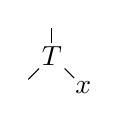
\begin{tikzpicture}[baseline=(T.base), inner sep=1pt]
      \node (T) {$T$};
      \node (x) at (.4,-.4) {$x$};
      \draw (T) -- (x);
      \draw (T) -- ++(-.3,-.3);
      \draw (T) -- ++(0,.35);
   \end{tikzpicture}
   \quad
	   \text{和}
   \quad
   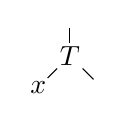
\begin{tikzpicture}[baseline=(T.base), inner sep=1pt]
      \node (T) {$T$};
      \node (x) at (-.4,-.4) {$x$};
      \draw (T) -- (x);
      \draw (T) -- ++(.3,-.3);
      \draw (T) -- ++(0,.35);
   \end{tikzpicture}
   \quad
	   \text{和}
   \quad
   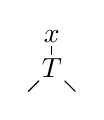
\begin{tikzpicture}[baseline=(T.base), inner sep=1pt]
      \node (T) {$T$};
      \node (x) at (0,.4) {$x$};
      \draw (T) -- (x);
      \draw (T) -- ++(.3,-.3);
      \draw (T) -- ++(-.3,-.3);
   \end{tikzpicture}
\]
%
要完全精确地说明每一种写法的含义，我们应该给边加上标签。
例如，我们会写成
$
   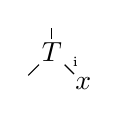
\begin{tikzpicture}[baseline=(T.base), inner sep=1pt]
      \node (T) {$T$};
      \node (x) at (.4,-.4) {$x$};
      \draw (T) -- (x) node[midway, above right, font=\tiny] {i};
      \draw (T) -- ++(-.3,-.3);
      \draw (T) -- ++(0,.3);
   \end{tikzpicture}
$
来表示矩阵 $\sum_i T_i x_i$。
不过，相关的边通常能从上下文中看出；这正是张量图记号比 Einstein 求和记号更清爽的原因之一。

\[
   Y_{i,j} = \sum_{k,l,m,n,o} A_{i,k} B_{l,n,o} C_{j,k,l,m} D_{m,n} E_o
   \quad
   \Leftrightarrow
   % \quad
   \vcenter{\hbox{
      \import{figures/}{basic_graph.pdf_tex}
   }}
\]

张量图的\emph{核心原则}是：\emph{边缩并满足结合律}。
这意味着你可以按任意喜欢的顺序缩并任意边。
从上面的求和表示也能看出这一点，因为其中对 $k,l,m,n$ 的求和可以按任意顺序重排。

不同缩并顺序的计算代价可能相差很大。
遗憾的是，寻找最优顺序在计算上并不容易。
关于寻找最佳缩并顺序的算法以及近似缩并方法，见第~\ref{sec:opt_contr} 节。

注意，张量图并不总是连通的。
我们已经看到，两个向量的外积可以写成
   $\begin{tikzpicture}[baseline=(a0.base), inner sep=1pt]
      \node (a0) {$a$};
      \node[right=.5em of a0] (a1) {$b$};
      \draw (a0.west) -- ++(-.3,0) node {};
      \draw (a1.east) -- ++(.3,0) node {};
   \end{tikzpicture}$.
从求和表示来看这很自然：没有边就意味着没有求和。
因此这里 $y_{i,j} = a_i b_j$，这正是外积 $y=a\otimes b$。
% Can also mention how this gives us scaling by letter (5) be the order-0 tensor with value 5.


\section{复制张量}

一个特别重要的张量是“复制”张量，也称为“对角”张量、“Kronecker delta”张量或“spider”张量。
最简单的版本是全 1 向量，我们把它写作 $\sbullet-$。
也就是说 $\sbullet_i = 1$。
一般的 $n$ 阶版本在对角线上取值为 1，在其他位置取值为 0：
\[
   \sbullet_{i,j,k,\ldots} = \begin{cases}
      1\quad \text{if } i=j=k=\dots \\
      0\quad \text {otherwise}
   \end{cases}
\]
% This is also known as the ``copy'' or ``spider'' tensor, or ``generalized Kronecker delta''.
或者，使用 Iverson 记号，\footnote{%
对一个逻辑命题 $P$，我们定义 $
   [P] = \begin{cases}
      1 \text{ if } P \\
      0 \text{ otherwise}
   \end{cases}
$.} $\sbullet_{i,j,k,\dots} = [i=j=k=\dots]$.
可以看到，2 阶复制张量 $-\sbullet- = I$ 只是单位矩阵，
因此可以像这样直接从图中删去：
\[-A\!-\!\sbullet\!-\!B- = -A\!-\!B-\]

高阶复制张量非常有用，因为它们让我们能够把简单的张量图变成超图。
一个简单的用法是表示对角矩阵 $D_a$，它在对角线上是 $a$，其他位置是 0。
我们可以写成
\[
   D_a = 
   \begin{tikzpicture}[baseline=(T.base), inner sep=1pt]
      \node (T) {$\sbullet$};
      \node (x) at (.3,-.3) {$a$};
      \draw (T) -- (x);
      \draw (T) -- ++(-.25,-.25);
      \draw (T) -- ++(0,.3);
   \end{tikzpicture}
\]
为什么？
因为 $(D_a)_{i,j} = \sum_k \sbullet_{i,j,k} a_k = \sum_k [i=j=k] a_k = [i=j] a_i$。
类似地，Hadamard 积 $(a\circ b)_i = a_i b_i$ 可以写成
\[
   a \circ b =
   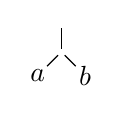
\begin{tikzpicture}[baseline=(T.base), inner sep=1pt]
      \node (T) {$\sbullet$};
      \node (a) at (-.3,-.3) {$a$};
      \node (b) at (.3,-.3) {$b$};
      \draw (T) -- (a);
      \draw (T) -- (b);
      \draw (T) -- ++(0,.3);
   \end{tikzpicture}
\]
现在，让我们看看为什么大家都喜欢复制张量：用“复制张量操作”来
证明恒等式 $D_aD_b = D_{a\circ b}$：
\[
   D_a D_b =
   \begin{tikzpicture}[baseline=(T.base), inner sep=1pt]
      \node (T) {$\sbullet$};
      \node (a) at (-.3,-.3) {$a$};
      \draw (T) -- (a);
      \node (T2) at (.5,0) {$\sbullet$};
      \node (b) at (.8,-.3) {$b$};
      \draw (T) -- ++(0,.3);
      \draw (T) -- (T2);
      \draw (T2) -- (b);
      \draw (T2) -- ++(0,.3);
   \end{tikzpicture}
   =
   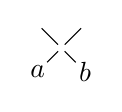
\begin{tikzpicture}[baseline=(T.base), inner sep=1pt]
      \node (T) {$\sbullet$};
      \node (a) at (-.3,-.3) {$a$};
      \node (b) at (.3,-.3) {$b$};
      \draw (T) -- (a);
      \draw (T) -- (b);
      \draw (T) -- ++(.25,.25);
      \draw (T) -- ++(-.25,.25);
   \end{tikzpicture}
   =
   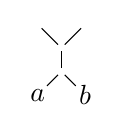
\begin{tikzpicture}[baseline=(T.base), inner sep=1pt]
      \node (T) {$\sbullet$};
      \node (a) at (-.3,-.3) {$a$};
      \node (b) at (.3,-.3) {$b$};
      \draw (T) -- (a);
      \draw (T) -- (b);
      \node (T2) at (0,.3) {$\sbullet$};
      \draw (T) -- (T2);
      \draw (T2) -- ++(.25,.25);
      \draw (T2) -- ++(-.25,.25);
   \end{tikzpicture}
   =
   D_{a\circ b}.
\]
你可以用求和表示来验证这一点。

这里起作用的一般规则是：任何由复制张量组成的连通子图都可以合并成一个复制张量。
有时我们甚至足够幸运，化简后还会留下一个可以删去的单位矩阵：
%\begin{figure}[h]
%   \centering{
   %\def\svgwidth{.5\linewidth}
   %\import{figures/}{path1.pdf_tex}
   %\\
\[
   \def\svgwidth{.75\linewidth}
   \import{figures/}{path2.pdf_tex}
   .
\]
%   \caption{Contracting copy tensors and identity matrices}
%   \label{fig:spiders}
%   }
%\end{figure}
唯一需要稍微小心的是结果张量为 0 阶的时候。
根据你如何定义 0 阶复制张量 $\sbullet$，恒等式 $\sbullet\!-\!\sbullet = \sbullet$ 可能成立，也可能不成立。

在普通向量记号中许多需要特殊记号的构造（例如对角矩阵或 Hadamard 积），都可以用复制张量统一起来。
%
在《Matrix Cookbook》中，他们定义了 4 阶张量 $J$，
它满足 $J_{i,j,k,l} = [i=k][j=l]$，我们会把它写成
$J=\vcenter{\hbox{
   \begin{tikzpicture}[inner sep=0pt]
   \node (a0) {$\sbullet$};
   \draw (a0.east) -- ++(.2,0);
   \draw (a0.west) -- ++(-.2,0);
   \node[below=.2em of a0] (a1) {$\sbullet$};
   \draw (a1.east) -- ++(.2,0);
   \draw (a1.west) -- ++(-.2,0);
\end{tikzpicture}}}$,
并且满足例如 $\frac{dX}{dX}=J$。
使用“张量积”，你可以写成 $J=I\otimes I$。
注意，$J$ 不同于 4 阶复制张量

\begin{tikzpicture}[baseline=(a0.base), inner sep=0pt]
   \node (a0) {$\sbullet$};
   \draw (a0) -- ++(.17,.17);
   \draw (a0) -- ++(.17,-.17);
   \draw (a0) -- ++(-.17,.17);
   \draw (a0) -- ++(-.17,-.17);
\end{tikzpicture}.

\section{张量求和}

张量积可以表示任何线性函数。
也就是说，满足 $f(a x, b y) = a b f(x,y)$ 的函数都可以这样表达。
不幸的是，并非所有张量上的操作都是线性的。
即使像两个向量之和 $x+y$ 这样简单的运算，也无法用一个简单的缩并图来表示。
（注意这不是线性的，因为 $ax+by\neq ab(x+y)$。）

为了处理这个重要操作，Penrose 建议直接把两个图写在一起，中间加一个加号，例如 $-x + -y$。
注意这本身仍然是 1 阶张量，尽管看起来像是有两条自由边。
如果我们想把这个和与另一个张量相乘，可以用括号写成 $-M\!-\!(-x + -y)$。

在处理求和时使用命名边会很有帮助，这样更容易看清哪些边彼此对应。
求和与张量积之间有很好的相互作用，满足一种广义的分配律：
%\begin{figure}[h]
%\centering{
%\def\svgwidth{\linewidth}
\[
\def\svgwidth{.75\linewidth}
\import{figures/}{path3.pdf_tex}
.
\]
%\caption{Distributive law}
%\label{fig:dist}
%}
%\end{figure}

当我们相加的张量边数不同，或者边名不同的时候，可以使用“广播（broadcasting）”。
%Say we want to add a matrix $\,_i\!-M-_j$ and a vector $x$.
假设我们想把一个矩阵 $M$ 和一个向量 $x$ 相加。
这到底是什么意思？
如果我们想把 $x$ 加到 $M$ 的每一行上，可以写成
$
\vcenter{\hbox{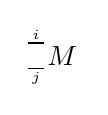
\begin{tikzpicture}[inner sep=1pt]
   \node (M) {$M$};
   \draw (M.north west) -- ++(-.2,0) node[midway, above, font=\tiny] {$i$};
   \draw (M.south west) -- ++(-.2,0) node[midway, below, font=\tiny] {$j$};
\end{tikzpicture}}}
+
\vcenter{\hbox{\begin{tikzpicture}[inner sep=1pt]
   \node (a0) {$\sbullet$};
   \draw (a0.west) -- ++(-.2,0) node[midway, above, font=\tiny] {$i$};
   \node[below=.2em of a0] (a1) {$x$};
   \draw (a1.west) -- ++(-.2,0) node[midway, below, font=\tiny] {$j$};
\end{tikzpicture}}}
$.
这是因为
$
\vcenter{\hbox{\begin{tikzpicture}[inner sep=1pt]
   \node (a0) {$\sbullet$};
   \draw (a0.west) -- ++(-.2,0) node[midway, above, font=\tiny] {$i$};
   \node[below=.2em of a0] (a1) {$x$};
   \draw (a1.west) -- ++(-.2,0) node[midway, below, font=\tiny] {$j$};
\end{tikzpicture}}}
$
这是 $x$ 与全 1 向量的外积，得到的是一个每一行都相同的矩阵。
类似地，如果我们想把 $x$ 加到每一列上，可以使用这个矩阵
$
\vcenter{\hbox{\begin{tikzpicture}[inner sep=1pt]
   \node (a0) {$\sbullet$};
   \draw (a0.west) -- ++(-.2,0) node[midway, below, font=\tiny] {$j$};
   \node[above=.2em of a0] (a1) {$x$};
   \draw (a1.west) -- ++(-.2,0) node[midway, above, font=\tiny] {$i$};
\end{tikzpicture}}}
$.

注意，处理张量时我们通常不谈“行”或“列”，而只是使用张量的边名（有时也叫轴）。
当使用命名边时，像“转置”这样的经典向量记号操作也可以去掉。
矩阵 $X^T$ 只是把左边和右边的边交换一下而已。
但如果边已经命名，我们就根本不必再去追踪“边在什么位置”了。

\section{转置}
在经典矩阵记号中，转置会交换矩阵的指标，因此
\[
   (A^T)_{ij} = A_{ji}.
\]
在张量图记号中，我们有两种选择，取决于是否要让边的位置具有意义。
当边位置有意义时，我们通常让“左边”对应第一个指标，让“右边”对应第二个指标。
因此转置就需要把边翻转：
\[
   (\matmul{A})^T
   =
   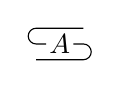
\begin{tikzpicture}[baseline=(a0.base), inner sep=1pt]
      \node (a0) {$A$};
      \draw (a0) -- ++(.3, 0) arc (270:90:-.1) --  ++(-.6, 0);
      \draw (a0) -- ++(-.3, 0) arc (270:90:.1) --  ++(.6, 0);
   \end{tikzpicture}
   =
   \matmul{A^T}.
\]
有些作者喜欢用把张量上下翻转的记号 $\matmul{\vflip{A}}$，作为交换左右边的更简洁写法。

在实际计算中，追踪边的位置很容易出错。
更稳妥的做法是给张量的“输出”命名，并让转置去重命名这些边：
\[
   (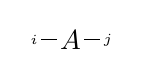
\begin{tikzpicture}[baseline=(A.base), inner sep=1pt]
   \node (A) {$A$};
   \draw (A.west) -- ++(-.2,0) node[left, font=\tiny] {$i$};
   \draw (A.east) -- ++(.2,0) node[right, font=\tiny] {$j$};
\end{tikzpicture})^T
=
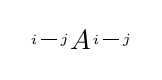
\begin{tikzpicture}[baseline=(A.base), inner sep=1pt]
   \node (A) {$A$};
   \node[font=\tiny] (i) at (-.2,0) {$j$};
   \node[font=\tiny] (j) at (.2,0) {$i$};
   \draw (i.west) -- ++(-.2,0) node[left, font=\tiny] {$i$};
   \draw (j.east) -- ++(.2,0) node[right, font=\tiny] {$j$};
\end{tikzpicture}
\]
%
重命名可以通过乘上单位矩阵来完成：
\[
(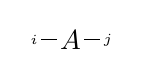
\begin{tikzpicture}[baseline=(A.base), inner sep=1pt]
   \node (A) {$A$};
   \draw (A.west) -- ++(-.2,0) node[left, font=\tiny] {$i$};
   \draw (A.east) -- ++(.2,0) node[right, font=\tiny] {$j$};
\end{tikzpicture})
(
\begin{tikzpicture}[baseline=(A.base), inner sep=1pt]
   \node (A) {$\sbullet$};
   \draw (A.west) -- ++(-.2,0) node[left, font=\tiny] {$j$};
   \draw (A.east) -- ++(.2,0) node[right, font=\tiny] {$k$};
\end{tikzpicture})
=
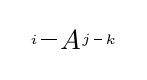
\begin{tikzpicture}[baseline=(A.base), inner sep=1pt]
   \node (A) {$A$};
   \draw (A.west) -- ++(-.2,0) node[left, font=\tiny] {$i$};
   \node[font=\tiny] (j) at (.2,0) {$j$};
   \draw (j) -- ++(.2,0) node[right, font=\tiny] {$k$};
\end{tikzpicture},
\]
但必须小心，因为重叠的边名会让乘法失去结合性。
例如：
\[
   \big[
(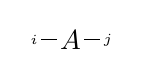
\begin{tikzpicture}[baseline=(A.base), inner sep=1pt]
   \node (A) {$A$};
   \draw (A.west) -- ++(-.2,0) node[left, font=\tiny] {$i$};
   \draw (A.east) -- ++(.2,0) node[right, font=\tiny] {$j$};
\end{tikzpicture})
(
\begin{tikzpicture}[baseline=(A.base), inner sep=1pt]
   \node (A) {$\sbullet$};
   \draw (A.west) -- ++(-.2,0) node[left, font=\tiny] {$j$};
   \draw (A.east) -- ++(.2,0) node[right, font=\tiny] {$k$};
\end{tikzpicture})
\big]
(
\begin{tikzpicture}[baseline=(A.base), inner sep=1pt]
   \node (A) {$\sbullet$};
   \draw (A.west) -- ++(-.2,0) node[left, font=\tiny] {$k$};
   \draw (A.east) -- ++(.2,0) node[right, font=\tiny] {$j$};
\end{tikzpicture})
=
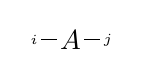
\begin{tikzpicture}[baseline=(A.base), inner sep=1pt]
   \node (A) {$A$};
   \draw (A.west) -- ++(-.2,0) node[left, font=\tiny] {$i$};
   \draw (A.east) -- ++(.2,0) node[right, font=\tiny] {$j$};
\end{tikzpicture}
\neq
(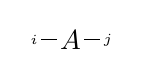
\begin{tikzpicture}[baseline=(A.base), inner sep=1pt]
   \node (A) {$A$};
   \draw (A.west) -- ++(-.2,0) node[left, font=\tiny] {$i$};
   \draw (A.east) -- ++(.2,0) node[right, font=\tiny] {$j$};
\end{tikzpicture})
   \big[
(
\begin{tikzpicture}[baseline=(A.base), inner sep=1pt]
   \node (A) {$\sbullet$};
   \draw (A.west) -- ++(-.2,0) node[left, font=\tiny] {$j$};
   \draw (A.east) -- ++(.2,0) node[right, font=\tiny] {$k$};
\end{tikzpicture})
(
\begin{tikzpicture}[baseline=(A.base), inner sep=1pt]
   \node (A) {$\sbullet$};
   \draw (A.west) -- ++(-.2,0) node[left, font=\tiny] {$k$};
   \draw (A.east) -- ++(.2,0) node[right, font=\tiny] {$j$};
\end{tikzpicture})
\big]
=
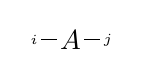
\begin{tikzpicture}[baseline=(A.base), inner sep=1pt]
   \node (A) {$A$};
   \draw (A.west) -- ++(-.2,0) node[left, font=\tiny] {$i$};
   \draw (A.east) -- ++(.2,0) node[right, font=\tiny] {$j$};
\end{tikzpicture}
\,
\begin{tikzpicture}[baseline=-0.6em, inner sep=1pt]
   \node (a0) {$\sbullet$};
   \node[below=.1 of a0] (a1) {$\sbullet$};
   \draw (a0) -- ++(.1, 0) arc (270:90:-.15) -- (a1);
   \draw (a1) -- ++(-.1, 0) arc (270:90:.15) -- (a0);
\end{tikzpicture},
\]
其中
$\begin{tikzpicture}[baseline=-0.7em, inner sep=1pt]
   \node (a0) {$\sbullet$};
   \node[below=.1 of a0] (a1) {$\sbullet$};
   \draw (a0) -- ++(.1, 0) arc (270:90:-.15) -- (a1);
   \draw (a1) -- ++(-.1, 0) arc (270:90:.15) -- (a0);
\end{tikzpicture}$
等于矩阵维数。
在 Tensorgrad 中，我们通过要求任何一个边名在任意乘积中最多出现两次来解决这个问题。

为了转写《Matrix Cookbook》，使用“位置有意义”的记号更方便。
我们注意到如下恒等式：
\begin{walign}
(A^T)^T &= A 
&
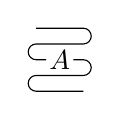
\begin{tikzpicture}[baseline=(a0.base), inner sep=1pt]
   \node (a0) {$A$};
   \draw (a0) -- ++(.3, 0) arc (270:90:-.1) -- ++(-.6, 0) arc (90:270:.1) -- ++(.6, 0);
   \draw (a0) -- ++(-.3, 0) arc (270:90:.1) -- ++(.6, 0) arc (90:270:-.1) -- ++(-.6, 0);
\end{tikzpicture}
&=
\matmul{A}
\\
%%%%%%%%%%%%%%%%%%%%%%%%%%%%%%%%%%%%%%%%%%%%%%%%%%%%%%%%%%%%%%%%%%%%%%%%%%%%%%%%
\tag{4}
(A + B)^T &= A^T + B^T
&
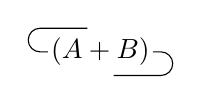
\begin{tikzpicture}[baseline=(a0.base), inner sep=1pt]
   \node (a0) {$\left( \matmul{A} + \matmul{B} \right)$};
   \draw (a0.east) -- ++(.1, 0) arc (270:90:-.15) -- ++(-.6, 0);
   \draw (a0.west) -- ++(-.1, 0) arc (270:90:.15) -- ++(.6, 0);
\end{tikzpicture}
&=
   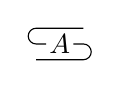
\begin{tikzpicture}[baseline=(a0.base), inner sep=1pt]
      \node (a0) {$A$};
      \draw (a0) -- ++(.3, 0) arc (270:90:-.1) --  ++(-.6, 0);
      \draw (a0) -- ++(-.3, 0) arc (270:90:.1) --  ++(.6, 0);
   \end{tikzpicture}
+
   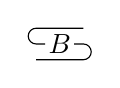
\begin{tikzpicture}[baseline=(a0.base), inner sep=1pt]
      \node (a0) {$B$};
      \draw (a0) -- ++(.3, 0) arc (270:90:-.1) --  ++(-.6, 0);
      \draw (a0) -- ++(-.3, 0) arc (270:90:.1) --  ++(.6, 0);
   \end{tikzpicture}
%\\
\end{walign}
\begin{walign}
%%%%%%%%%%%%%%%%%%%%%%%%%%%%%%%%%%%%%%%%%%%%%%%%%%%%%%%%%%%%%%%%%%%%%%%%%%%%%%%%
\tag{5}
(AB)^T &= B^T A^T
&
   \begin{tikzpicture}[baseline=(a.base), inner sep=1pt]
      \node (a) {$A$};
      \node[right=.5em of a] (b) {$B$};
      \draw (a) -- (b);
      \draw (b) -- ++(.3, 0) arc (270:90:-.1) --  ++(-.6, 0);
      \draw (a) -- ++(-.3, 0) arc (270:90:.1) --  ++(.6, 0);
   \end{tikzpicture}
&=
\begin{tikzpicture}[baseline=-.8em, inner sep=1pt]
   \node (a) {\vflip{$A$}};
   \node[below=.3em of a] (b) {\vflip{$B$}};
   \draw (a) -- ++(.3, 0);
   \draw (a) -- ++(-.3, 0) arc (90:270:.1) -- ++(.6, 0) arc (270:90:-.1) -- (b);
   \draw (b) -- ++(-.3, 0);
\end{tikzpicture}
=
\matmul{ \vflip{B}, \vflip{A} }
\end{walign}

\subsection{高阶情形}
可以把转置的思想推广到高阶张量。
这需要把边划分为“输入”和“输出”边，更常见地说，就是“逆变”边和“协变”边。
关于这一点的更多内容，见本章末尾的小节。

如果 $A^T = A$，我们就说矩阵是对称的。
对于高阶张量，对称的方式有很多种。
更多内容见第~\ref{sec:symmetry} 节。

\section{迹}

方阵的“迹”定义为 $\mathrm{Tr}(A) = \sum_i A_{i,i}$。
在张量图记号中，这对应一条自环边：$\trace{A}{1}$。
《Matrix Cookbook》中有一系列使用迹的恒等式。
我们用张量图把它们重写出来：
\begin{walign}
   \tag{11}
   \sum_{i=1}^{n} A_{ii} &= \mathrm{Tr}(A) = \mathrm{Tr}(A I)
   &
   \trace{A}{1} &= \trace{A, \sbullet}{2}
   \\
   %%%%%%%%%%%%%%%%%%%%%%%%%%%%%%%%%%%%%%%%
   \tag{13}
   \mathrm{Tr}(A) &= \mathrm{Tr}(A^T)
   &
   \trace{A}1
   \hspace{-1em}
   &=
   \hspace{-1em}
   \vflip{\trace{A}1}
   \\[0.5em]
   %%%%%%%%%%%%%%%%%%%%%%%%%%%%%%%%%%%%%%%%
   \tag{14}
   \mathrm{Tr}(AB)
   &=
   \mathrm{Tr}(BA)
   &
   \trace{A,B}2
   \hspace{-.5em}
   &=
   \hspace{.5em}
   \begin{tikzpicture}[baseline=-1em, inner sep=1pt]
      \node (a) {$\vflip{B}$};
      \node[below=.3em of a] (b) {$A$};
      \draw (a) -- ++(-.3, 0) arc (90:270:.2) -- (b);
      \draw (a) -- ++(.3, 0) arc (270:90:-.2) -- (b);
   \end{tikzpicture}
   \hspace{.5em}
   =
   \hspace{-.5em}
   \trace{B,A}2
   \\[0.5em]
   %%%%%%%%%%%%%%%%%%%%%%%%%%%%%%%%%%%%%%%%
   \tag{15}
   \mathrm{Tr}(A+B)
   &= \mathrm{Tr}(A) + \mathrm{Tr}(B)
   &
   %\trace{(A+B),\sbullet}1
   %\trace{(\matmul{A}+\matmul{B}),\sbullet}1
   %\trace{(\matmul{A}+\matmul{B})}1
   %\trace{(\matmul{A}+\matmul{B}),\sbullet}{2}
   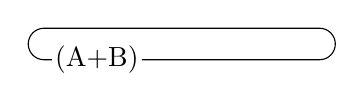
\begin{tikzpicture}[baseline=(a.base), inner sep=1pt]
      \node (a) {(\matmul{A}+\matmul{B})};
      \draw (a.west) -- ++(-.1, 0) arc (270:90:.2) -- ++(3.5, 0) arc (270:90:-.2) -- (a.east);
   \end{tikzpicture}
   &=
   \hspace{-1em}
   \trace{A}1
   \hspace{-1em}
   +
   \hspace{-1em}
   \trace{B}1
   \hspace{-1em}
   \\[0.5em]
   %%%%%%%%%%%%%%%%%%%%%%%%%%%%%%%%%%%%%%%%
   \tag{16}
   \mathrm{Tr}(ABC) &= \mathrm{Tr}(BCA)
   &
   \trace{A,B,C}1 &= \trace{B,C,A}1
   \\
                  & = \mathrm{Tr}(CAB)
                  &&= \trace{C,A,B}1
   \\[0.5em]
   %%%%%%%%%%%%%%%%%%%%%%%%%%%%%%%%%%%%%%%%
   \tag{17}
   a^T a &= \mathrm{Tr}(a a^T)
   &
   \vecmatvec{1em}{a}{}{a}
   &=
   \mathrm{Tr}(
   \begin{tikzpicture}[baseline=(a0.base), inner sep=1pt]
      \node (a0) {$a$};
      \node[right=.5em of a0] (a1) {$a$};
      \draw (a0.west) -- ++(-.3,0) node {};
      \draw (a1.east) -- ++(.3,0) node {};
   \end{tikzpicture}
   )
 \\&&&=
   \hspace{-1em}
   \begin{tikzpicture}[baseline=(a0.base), inner sep=1pt]
      \node (a0) {$a$};
      \node[right=1em of a0] (a1) {$a$};
      \path (a0) edge [out=160, in=20, looseness=2] (a1);
   \end{tikzpicture}
   \hspace{-1em}
\end{walign}

\subsection{高阶迹}
对于高阶张量，我们仍然把迹定义为对角元素之和。
也就是说，对于一个 $n$ 阶张量 $A$，迹就是它与 $n$ 阶复制张量的乘积：
\[
   \begin{tikzpicture}[baseline=(T.base), inner sep=1pt]
      \node (Tr) {Tr(};
      \node[right=.3em of Tr] (T) {$T$};
      \node[right=.3em of T] (p) {)};
      \draw (T) -- ++(.3,-.3);
      \draw (T) -- ++(-.3,-.3);
      \draw (T) -- ++(0,.35);
   \end{tikzpicture}
   =
   \begin{tikzpicture}[baseline=(T.base), inner sep=1pt]
      \node (T) {$T$};
      \node[right=2em of T] (s) {$\sbullet$};
      \path (T) edge [out=90, in=120] (s);
      \path (T) edge [out=-30, in=200] (s);
      \path (T) edge [out=-120, in=220] (s);
   \end{tikzpicture}
   .
\]
在量子力学中，常会用到“部分迹”，我们可以用指标记号来定义：
\[
   \begin{tikzpicture}[baseline=(T.base), inner sep=1pt]
      \node (Tr) {Tr$_{i,j}$(};
      \node[right=.3em of Tr] (T) {$T$};
      \node[right=.3em of T] (p) {)};
      \draw (T) -- ++(.3,-.3) node[midway, below left, font=\tiny] {j};
      \draw (T) -- ++(-.3,-.3) node[midway, below right, font=\tiny] {i};
      \draw (T) -- ++(0,.35) node[midway, above right, font=\tiny] {k};
   \end{tikzpicture}
   =
   \hspace{-.5em}
   \begin{tikzpicture}[baseline=(T.base), inner sep=1pt]
      \node (T) {$T$};
      \draw (T) -- ++(0,.35) node[midway, above right, font=\tiny] {k};
      \path (T) edge [out=-120, in=-60, loop] (T);
   \end{tikzpicture}
   .
\]
当然，在张量图里，我们也可以不命名指标就使用部分迹。
我们甚至不必去想所做的缩并到底是不是迹。

\section{特征值}
特征值和特征向量是线性代数中的基本概念，在张量网络理论中也有重要应用。张量图记号可以把这些概念直观地表示出来。

对于矩阵 $A$，如果存在非零向量 $v$ 和标量 $\lambda$ 使得 $Av = \lambda v$，那么 $\lambda$ 就称为 $A$ 的一个特征值，而 $v$ 是相应的特征向量。
在张量图记号中，把它的特征分解写成 $A = Q\Lambda Q^{-1}$ 很方便，其中 $Q$ 的列是 $A$ 的特征向量，$\Lambda$ 是由特征值组成的对角矩阵。
因此：
\begin{align}
   \label{eq:eigen-decomposition}
   \begin{tikzpicture}[baseline=(A.base), inner sep=1pt]
   \node (A) {$A$};
   \draw (A.west) -- ++(-.3, 0);
   \draw (A.east) -- ++(+.3, 0);
   \end{tikzpicture}
   =
   \begin{tikzpicture}[baseline=(Q.base), inner sep=1pt]
   \node (Q) {$Q$};
   \draw (Q.west) -- ++(-.3, 0);
   \node[right=1em of Q] (dot) {$\sbullet$};
   \path (Q) edge (dot);
   \node[below=.3em of dot] (e) {$\lambda$};
   \path (dot) edge (e);
   \node[right=1em of dot] (Qi) {$Q^{-1}$};
   \path (dot) edge (Qi);
   \draw (Qi.east) -- ++(.3, 0);
   \end{tikzpicture}
\end{align}
矩阵的迹等于其特征值之和。我们可以用张量图表示这一关系：
\[
   \tag{12}
   \text{Tr}(A)
   =
   \hspace{-1em}
   \trace{A}{1}
   \hspace{-1em}
   =
   \hspace{-3em}
   \begin{tikzpicture}[baseline=(Q.base), inner sep=1pt]
      \node (Q) {$Q$};
      \node[right=1em of Q] (dot) {$\sbullet$};
      \path (Q) edge (dot);
      \node[below=.3em of dot] (e) {$\lambda$};
      \path (dot) edge (e);
      \node[right=1em of dot] (Qi) {$Q^{-1}$};
      \path (dot) edge (Qi);
      \path (Q.west) edge [out=160, in=20, looseness=2] (Qi.east);
   \end{tikzpicture}
   \hspace{-3em}
   =
   \hspace{-1em}
   \begin{tikzpicture}[baseline=(dot.base), inner sep=1pt]
      \node (dot) {$\sbullet$};
      \node[below=.3em of dot] (e) {$\lambda$};
      \path (dot) edge (e);
      \path (dot) edge [out=160, in=20, loop] ();
   \end{tikzpicture}
   \hspace{-1em}
   =
   \begin{tikzpicture}[baseline=(dot.base), inner sep=1pt]
      \node (dot) {$\sbullet$};
      \node[below=.3em of dot] (e) {$\lambda$};
      \path (dot) edge (e);
   \end{tikzpicture}
   =
   \sum_i \lambda_i
\]



\section{对称与对称化}
\label{sec:symmetry}

张量的一个常见性质是对称性。
对矩阵来说，对称性意味着 $A^T = A$。
对张量来说，则意味着交换其指标不会改变它的值。
典型例子是协方差矩阵或 Hessian 矩阵，
但某些高阶统计矩，比如三阶或四阶矩张量，也可能具有对称性。
有时这种对称性只相对于某个特定群成立，但大多数时候是相对于边的所有置换成立。
复制张量就是一个完全对称张量的简单例子。

有时我们会通过对所有指标置换求和来对张量进行对称化。
我们用一条波浪线覆盖被对称化的边来表示：
\[
   \begin{tikzpicture}[baseline=.1em, inner sep=2pt, x=1em, y=.7em]
      \draw (0,0) -- ++(1,0);
      \draw (0,1) -- ++(1,0);
      \draw [very thick, line width=2pt, decorate, decoration={snake, amplitude=0.5mm, segment length=2.5mm}] (0.5,-.7) to (0.5,1.7);
   \end{tikzpicture}
   =
   \begin{tikzpicture}[baseline=.1em, inner sep=2pt, x=1em, y=.7em]
      \draw (0,0) -- ++(1,0);
      \draw (0,1) -- ++(1,0);
   \end{tikzpicture}
   +
   \begin{tikzpicture}[baseline=.1em, inner sep=2pt, x=1em, y=.7em]
      \draw (0,0) -- ++(1,1);
      \draw (0,1) -- ++(1,-1);
   \end{tikzpicture}
   ,\quad
   \begin{tikzpicture}[baseline=.5em, inner sep=2pt, x=1em, y=.7em]
      \draw (0,0) -- ++(1,0);
      \draw (0,1) -- ++(1,0);
      \draw (0,2) -- ++(1,0);
      \draw [very thick, line width=2pt, decorate, decoration={snake, amplitude=0.5mm, segment length=2.5mm}] (0.5,-.7) to (0.5,2.7);
   \end{tikzpicture}
   =
   \begin{tikzpicture}[baseline=.5em, inner sep=2pt, x=1em, y=.7em]
      \draw (0,0) -- ++(1,0);
      \draw (0,1) -- ++(1,0);
      \draw (0,2) -- ++(1,0);
   \end{tikzpicture}
   +
   \begin{tikzpicture}[baseline=.5em, inner sep=2pt, x=1em, y=.7em]
      \draw (0,0) -- ++(1,0);
      \draw (0,1) -- ++(1,1);
      \draw (0,2) -- ++(1,-1);
   \end{tikzpicture}
   +
   \begin{tikzpicture}[baseline=.5em, inner sep=2pt, x=1em, y=.7em]
      \draw (0,0) -- ++(1,1);
      \draw (0,1) -- ++(1,-1);
      \draw (0,2) -- ++(1,0);
   \end{tikzpicture}
   +
   \begin{tikzpicture}[baseline=.5em, inner sep=2pt, x=1em, y=.7em]
      \draw (0,0) -- ++(1,1);
      \draw (0,1) -- ++(1,1);
      \draw (0,2) -- ++(1,-2);
   \end{tikzpicture}
   +
   \begin{tikzpicture}[baseline=.5em, inner sep=2pt, x=1em, y=.7em]
      \draw (0,0) -- ++(1,2);
      \draw (0,1) -- ++(1,-1);
      \draw (0,2) -- ++(1,-1);
   \end{tikzpicture}
   +
   \begin{tikzpicture}[baseline=.5em, inner sep=2pt, x=1em, y=.7em]
      \draw (0,0) -- ++(1,2);
      \draw (0,1) -- ++(1,0);
      \draw (0,2) -- ++(1,-2);
   \end{tikzpicture}
\]
例如，如果 $A$ 是一个方阵，
\(
   A + A^T =
   \begin{tikzpicture}[baseline=(A.base), inner sep=2pt, x=2em, y=2em]
      \node (A) at (0,0) {$A$};
      \draw (A) -- ++(-1,0);
      \draw (A) -- ++(1,0);
    \draw [very thick, decorate, decoration={snake, amplitude=.5mm, segment length=2.1mm}]
        ($(A)+(.6,-.3)$) arc [start angle=-20, end angle=200, x radius=0.6, y radius=0.5];
   \end{tikzpicture}
   =
   \begin{tikzpicture}[baseline=(A.base), inner sep=2pt, x=1.5em, y=2em]
      \node (A) at (0,0) {$A$};
      \draw (A) -- ++(-1,0);
      \draw (A) -- ++(1,0);
   \end{tikzpicture}
   +
   \begin{tikzpicture}[baseline=(a0.base), inner sep=1pt]
      \node (a0) {$A$};
      \draw (a0) -- ++(.3, 0) arc (270:90:-.1) --  ++(-.6, 0);
      \draw (a0) -- ++(-.3, 0) arc (270:90:.1) --  ++(.6, 0);
   \end{tikzpicture}
   .
\)
还有一个互补概念是\emph{反对称化}（或\emph{斜对称化}），此时我们对\emph{所有置换按适当符号}求和。
例如，一个 2 阶斜对称矩阵 \(A\) 满足 \(A_{ij} = -A_{ji}\)。
我们可以用一条扁平的粗线表示反对称化：
\(
   \begin{tikzpicture}[baseline=(A.base), inner sep=2pt, x=2em, y=2em]
      \node (A) at (0,0) {$A$};
      \draw (A) -- ++(-1,0);
      \draw (A) -- ++(1,0);
    \draw [very thick] ($(A)+(.6,-.2)$) arc [start angle=-10, end angle=190, x radius=0.6, y radius=0.5];
   \end{tikzpicture}
   =
   \begin{tikzpicture}[baseline=(A.base), inner sep=2pt, x=1.5em, y=2em]
      \node (A) at (0,0) {$A$};
      \draw (A) -- ++(-1,0);
      \draw (A) -- ++(1,0);
   \end{tikzpicture}
   -
   \begin{tikzpicture}[baseline=(a0.base), inner sep=1pt]
      \node (a0) {$A$};
      \draw (a0) -- ++(.3, 0) arc (270:90:-.1) --  ++(-.6, 0);
      \draw (a0) -- ++(-.3, 0) arc (270:90:.1) --  ++(.6, 0);
   \end{tikzpicture}
   .
\)
在更高阶的情形下，每一项的符号由置换的奇偶性决定。

这两种张量都是幂等的，因为对一个已经对称的张量再做对称化不会改变它：
\[
   \begin{tikzpicture}[baseline=.5em, inner sep=2pt, x=1em, y=.7em]
      \draw (0,0) -- ++(2,0);
      \draw (0,1) -- ++(2,0);
      \draw (0,2) -- ++(2,0);
      \draw [very thick, line width=2pt, decorate, decoration={snake, amplitude=0.5mm, segment length=2.5mm}] (0.66,-.7) to (0.66,2.7);
      \draw [very thick, line width=2pt, decorate, decoration={snake, amplitude=0.5mm, segment length=2.5mm}] (1.33,-.7) to (1.33,2.7);
   \end{tikzpicture}
   =
   \begin{tikzpicture}[baseline=.5em, inner sep=2pt, x=1em, y=.7em]
      \draw (0,0) -- ++(1,0);
      \draw (0,1) -- ++(1,0);
      \draw (0,2) -- ++(1,0);
      \draw [very thick, line width=2pt, decorate, decoration={snake, amplitude=0.5mm, segment length=2.5mm}] (0.5,-.7) to (0.5,2.7);
   \end{tikzpicture}
   ,\quad
   \begin{tikzpicture}[baseline=.5em, inner sep=2pt, x=1em, y=.7em]
      \draw (0,0) -- ++(2,0);
      \draw (0,1) -- ++(2,0);
      \draw (0,2) -- ++(2,0);
      \draw [very thick] (0.66,-.7) to (0.66,2.7);
      \draw [very thick] (1.33,-.7) to (1.33,2.7);
   \end{tikzpicture}
   =
   \begin{tikzpicture}[baseline=.5em, inner sep=2pt, x=1em, y=.7em]
      \draw (0,0) -- ++(1,0);
      \draw (0,1) -- ++(1,0);
      \draw (0,2) -- ++(1,0);
      \draw [very thick] (0.5,-.7) to (0.5,2.7);
   \end{tikzpicture}
   .
\]


\section{协变与逆变}

在物理学中，经常需要在不同坐标系之间变换。
这类变换往往会以不同方式作用在矩阵的左侧和右侧，也会类似地作用于行向量和列向量。
对于张量，这就推广为协变与逆变的概念。
借助这些概念，我们需要跟踪“输入”和“输出”向量。
我们还需要区分诸如单位矩阵 $\matmul{\sbullet}$、
$\begin{tikzpicture}[baseline=(a0.base), inner sep=0pt]
   \node (a0) {$\sbullet$};
   \draw (a0) -- ++(-.17,.1);
   \draw (a0) -- ++(-.17,-.1);
\end{tikzpicture}$,
and
$\begin{tikzpicture}[baseline=(a0.base), inner sep=0pt]
   \node (a0) {$\sbullet$};
   \draw (a0) -- ++(.17,.1);
   \draw (a0) -- ++(.17,-.1);
\end{tikzpicture}$.

这个概念让我们可以通过把输入边连接到输出边，像处理矩阵和向量那样在一定程度上“代数地”组合张量。
不过，对更复杂的张量来说，我们需要知道具体该连接哪些边，而这时指标记号更有用。

在计算机科学和机器学习中，协变与逆变的概念通常并不实用，所以本书不会使用它。

\section{练习}
\begin{exercise}
   给定一列矩阵 $A_1, A_2, \ldots, A_n \in \mathbb R^{n\times n}$，
   以及向量 $v_1, v_2, \ldots, v_n \in \mathbb R^n$，
   请用张量图画出由向量 $A_1v_1, A_2v_2, \ldots, A_nv_n$ 组成的矩阵。
\end{exercise}
\begin{exercise}
用张量图表示两个矩阵的 Hadamard 积（逐元素乘法）。
它与普通矩阵乘法有何不同？
（关于这一点，见 \ref{sec:hadamard}。）
\end{exercise}
\begin{exercise}
用张量图表示矩阵 $A = U\Sigma V^T$ 的 SVD。
这与特征分解的图示相比如何？
如何把它推广到高阶张量？
（在第 \ref{sec:HOSVD} 节我们会看到更多内容。）
\end{exercise}
